%----------------------------------------------------------------------------------------
%	PACKAGES AND THEMES
%----------------------------------------------------------------------------------------
\documentclass[aspectratio=169,xcolor=dvipsnames]{beamer}
\usetheme{SimplePlusAIC}
\usepackage{xcolor}
\usepackage{hyperref}
\usepackage{graphicx} % Allows including images
\usepackage{booktabs} % Allows the use of \toprule, \midrule and  \bottomrule in tables
\usepackage{svg} %allows using svg figures
\usepackage{tikz}
\usepackage{makecell}
\newcommand*{\defeq}{\stackrel{\text{def}}{=}}
\usefonttheme[onlymath]{serif}
\usepackage{mwe,tikz}\usepackage[percent]{overpic}
\usepackage{animate}

\usepackage{subcaption}
%Select the Epilogue font (requires luaLatex or XeLaTex compilers)
\usepackage{fontspec}
\setsansfont{Epilogue}[
    Path=./epilogueFont/,
    Scale=0.9,
    Extension = .ttf,
    UprightFont=*-Regular,
    BoldFont=*-Bold,
    ItalicFont=*-Italic,
    BoldItalicFont=*-BoldItalic
    ]
\newcommand{\vect}[1]{\mathbf{#1}}
%----------------------------------------------------------------------------------------
%	TITLE PAGE
%----------------------------------------------------------------------------------------

\title[short title]{Optimální tvar stěn idealizovaného\\ kavopulmonálního spojení} % The short title appears at the bottom of every slide, the full title is only on the title page
\subtitle{Diplomová práce}

\author[Surname]{Jan Bureš\textmd{, Radek Fučík, Radomír Chabiniok}}
\institute[KM FJFI 2024]{Katedra matematiky \newline Fakulta jaderná a fyzikálně inženýrská\newline České vysoké učení technické v Praze}
% Your institution as it will appear on the bottom of every slide, maybe shorthand to save space


\date{29. ledna 2025} % Date, can be changed to a custom date

%----------------------------------------------------------------------------------------
%	PRESENTATION SLIDES
%----------------------------------------------------------------------------------------

\begin{document}

\begin{frame}[plain, noframenumbering]
    % Print the title page as the first slide
    \vspace{-21mm}
    \titlepage
\end{frame}

\begin{frame}[plain, noframenumbering]{Přehled}
    % Throughout your presentation, if you choose to use \section{} and \subsection{} commands, these will automatically be printed on this slide as an overview of your presentation
    \tableofcontents
\end{frame}

%------------------------------------------------
\section{Motivace}
%------------------------------------------------

\begin{frame}{Motivační úloha}
	\begin{columns}[T] % align columns
		\begin{column}{.63\textwidth}
			\begin{figure}
				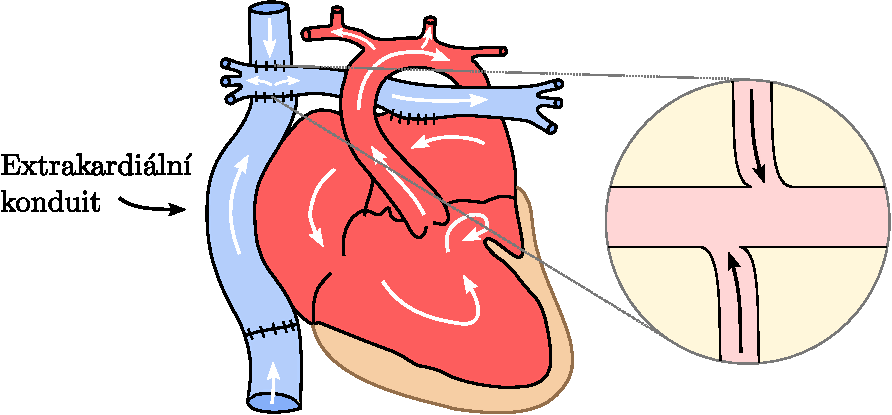
\includegraphics[width=0.9\linewidth]{Images/srdce_zoom_cz.pdf}
			\end{figure}
		\end{column}%
		\hfill%
		\begin{column}{.37\textwidth}
			\vspace{0pt}
			\textbf{Optimalizační úloha:}\\
			\vspace{6pt}
			Nalézt minimum
			\begin{equation*}
				\min _{\vect{x} \in \mathbb{X} } f \ (\vect{x}),
			\end{equation*}
			kde $ f \ (\vect{x}) $ je účelová funkce.\\
			\vspace{11pt}
			\textbf{Charakterizace:}\\[2pt]
			\begin{itemize}
				\item nelineární
				\item s vazbami
			\end{itemize}
		\end{column}%
	\end{columns}
\end{frame}

%------------------------------------------------
\section{Optimalizační rámec}
%------------------------------------------------
\begin{frame}{Rámec}
	
	\begin{figure}
		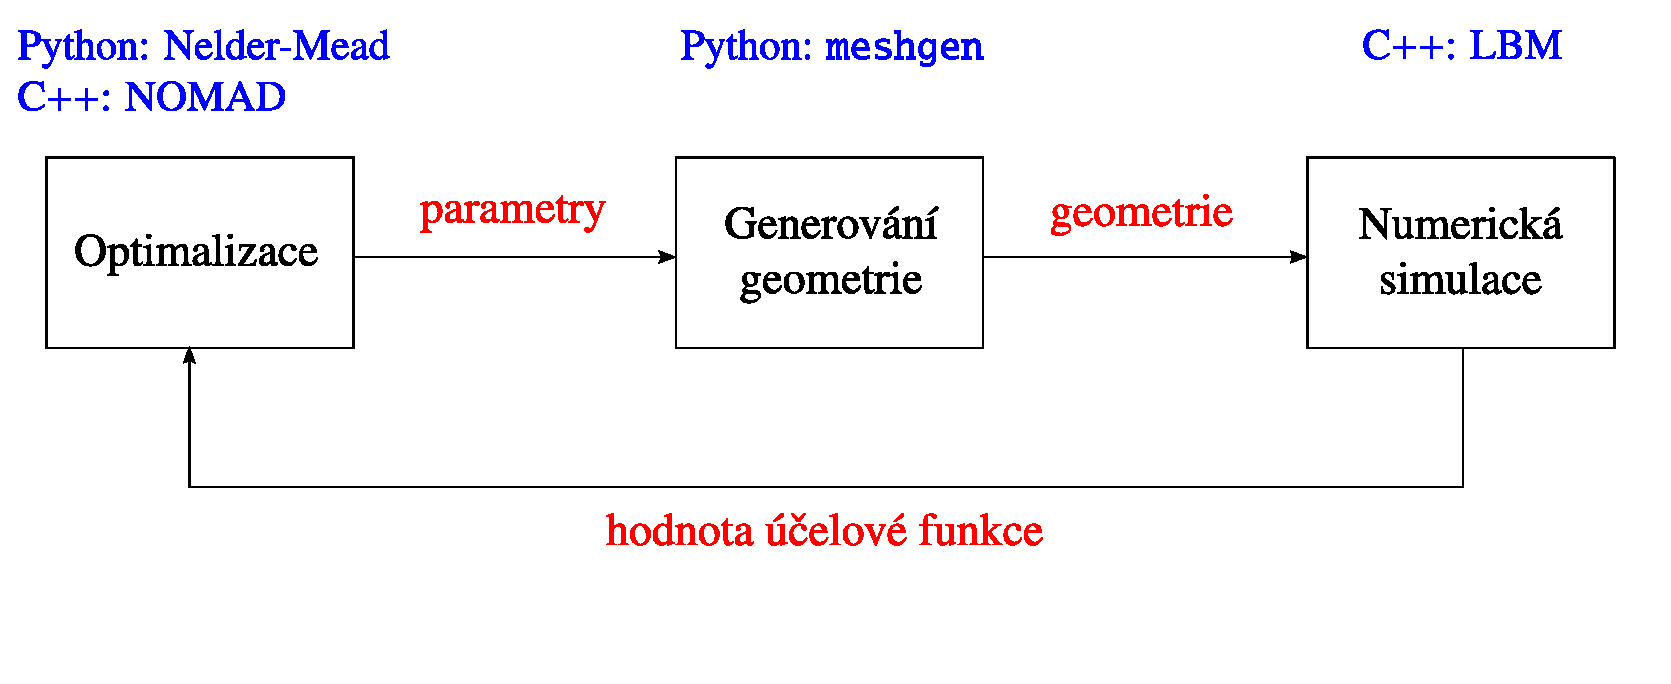
\includegraphics[width=0.95\linewidth, trim={0 -0.1cm 0 0}, clip]{Images/framework-cz.pdf}
	\end{figure}
\end{frame}
%------------------------------------------------
\begin{frame}{Rámec}
	\addtocounter{framenumber}{-1}
	\begin{figure}
		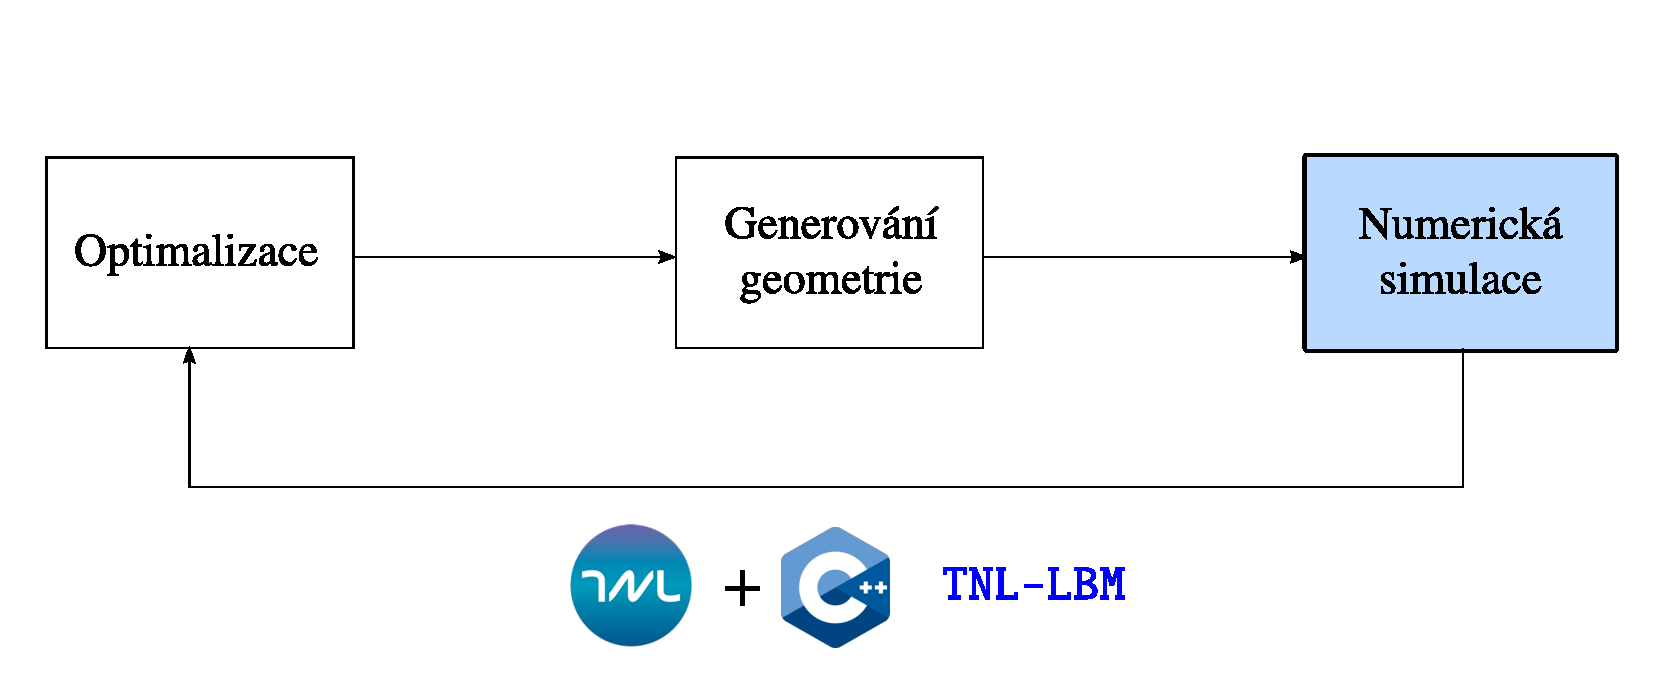
\includegraphics[width=0.95\linewidth, trim={0 -0.1cm 0 0}, clip]{Images/framework-cz-1.pdf}
	\end{figure}
\end{frame}
%------------------------------------------------
\begin{frame}{Mřížková Boltzmannova metoda}
	\begin{columns}[T] % align columns
		\begin{column}{.45\textwidth}
			\textbf{LBM:} - KM FJFI\\
			\begin{itemize}
				\item rychlostní model D3Q27, CuLBM
			\end{itemize}
		\begin{eqnarray*}
			\rho &=& \sum_{k=1}^{27} \varphi_{k}\\
			\rho \vect{u} &=& \sum_{k=1}^{27} \varphi_{k} \boldsymbol{\xi}_{k} + \dfrac{\Delta t}{2} \rho \boldsymbol{g}
		\end{eqnarray*}
			\textbf{Okrajové a počáteční podmínky:}\\
			\begin{itemize}
				\item konstatní přítok a free outflow OP
				\item hranice objektu $ \rightarrow $ bounce-back
				\item rovnovážná počáteční podmínka
			\end{itemize}
		\end{column}%
		\begin{column}{.5\textwidth}
			\textbf{Rovnice dynamiky tekutin:}
			\vspace{-13pt}
			\begin{center}
				$$\frac{\partial \rho}{\partial t} + \nabla \cdot (\rho \vect{u}) = 0 $$
				$$\frac{\partial (\rho \vect{u})}{\partial t} + \nabla \cdot (\rho \vect{u} \otimes \vect{u}) = \nabla \cdot \mathbf{T} + \rho \boldsymbol{g}$$
			\end{center}%
			\vspace{11pt}
			\textbf{Předpoklady:}\\[2pt]
			\begin{itemize}
				\item izotermální systém bez vnějších sil
				\item nestlačitelná newtonovská tekutina
			\end{itemize}
		\end{column}%
	\end{columns}
\end{frame}
%%------------------------------------------------
\begin{frame}{Rámec}
	\addtocounter{framenumber}{-1}
	\begin{figure}
		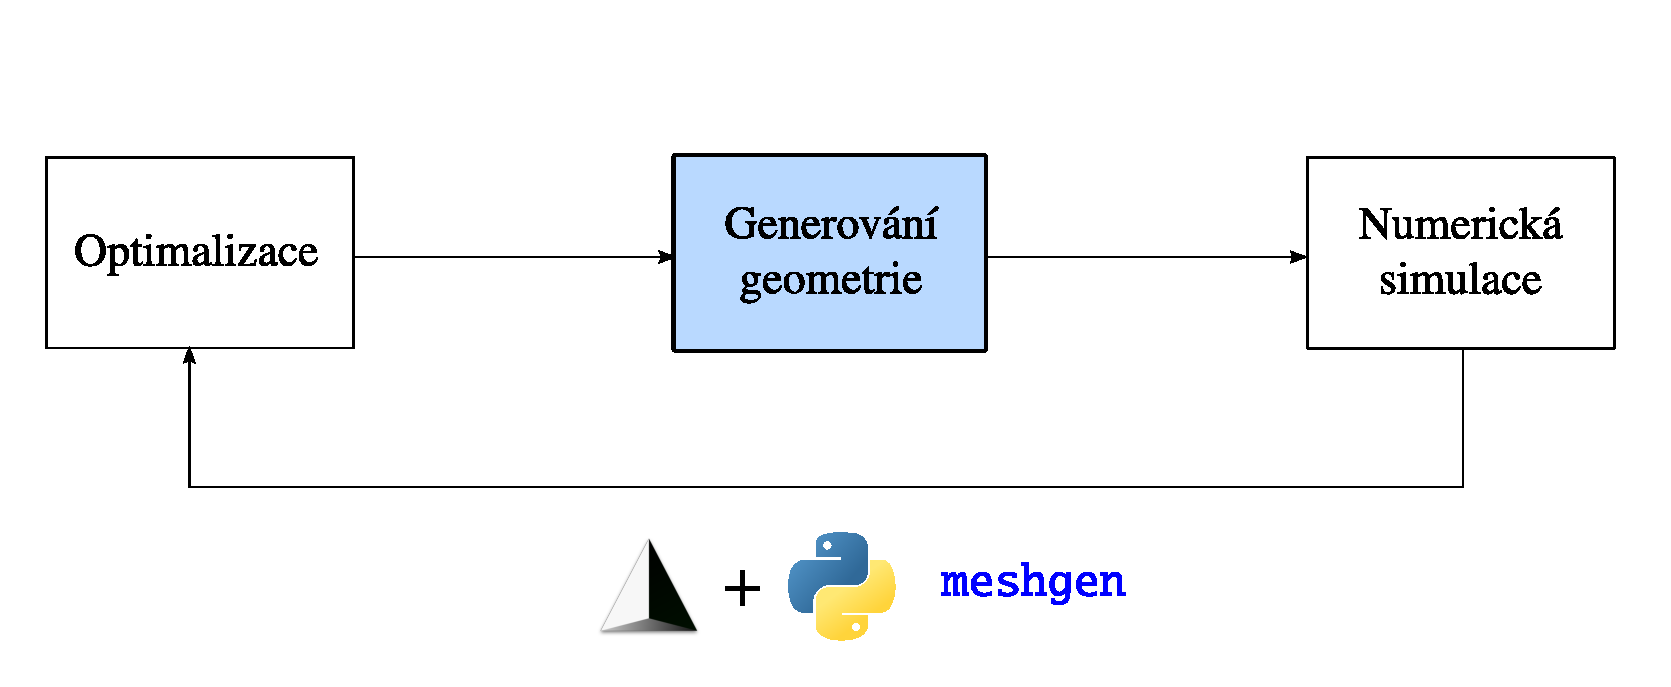
\includegraphics[width=0.95\linewidth, trim={0 -0.1cm 0 0}, clip]{Images/framework-cz-2.pdf}
	\end{figure}
\end{frame}
%------------------------------------------------
\begin{frame}{Generování geometrie}
	\begin{itemize}
		\item balík vytvořený pro účely parametrického generování geometrie a následné voxelizace
	\end{itemize}
	\begin{figure}
		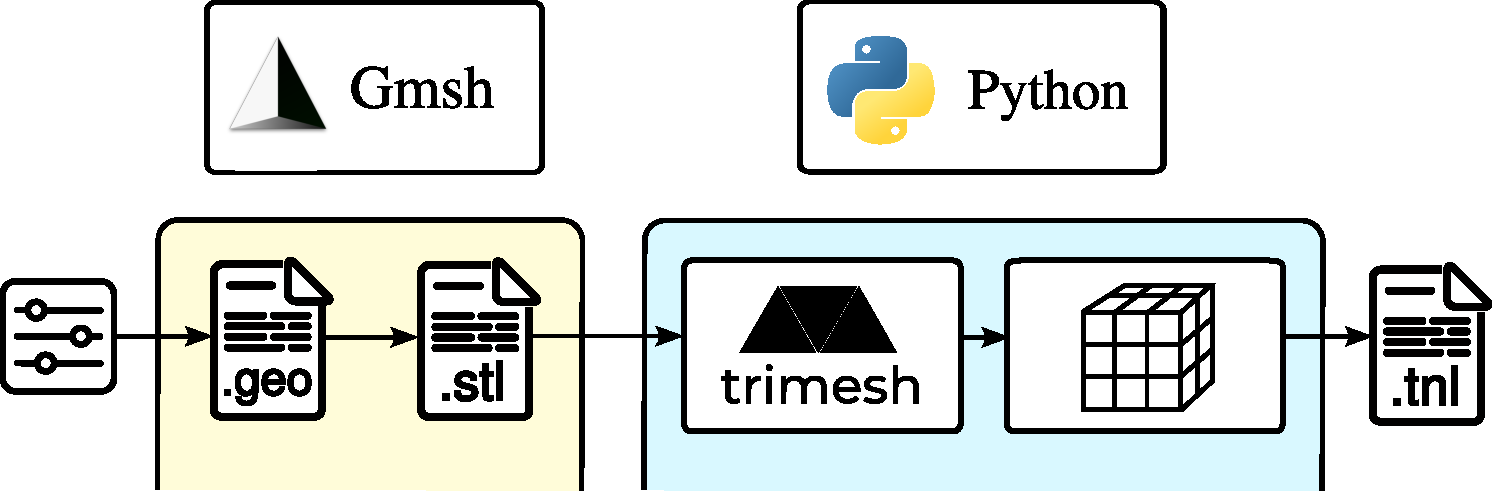
\includegraphics[width=0.8\linewidth, trim={0 -0.1cm 0 0}, clip]{Images/meshgen.pdf}
	\end{figure}
\end{frame}
%------------------------------------------------
\begin{frame}{Generování geometrie - šablona}
	\begin{figure}
		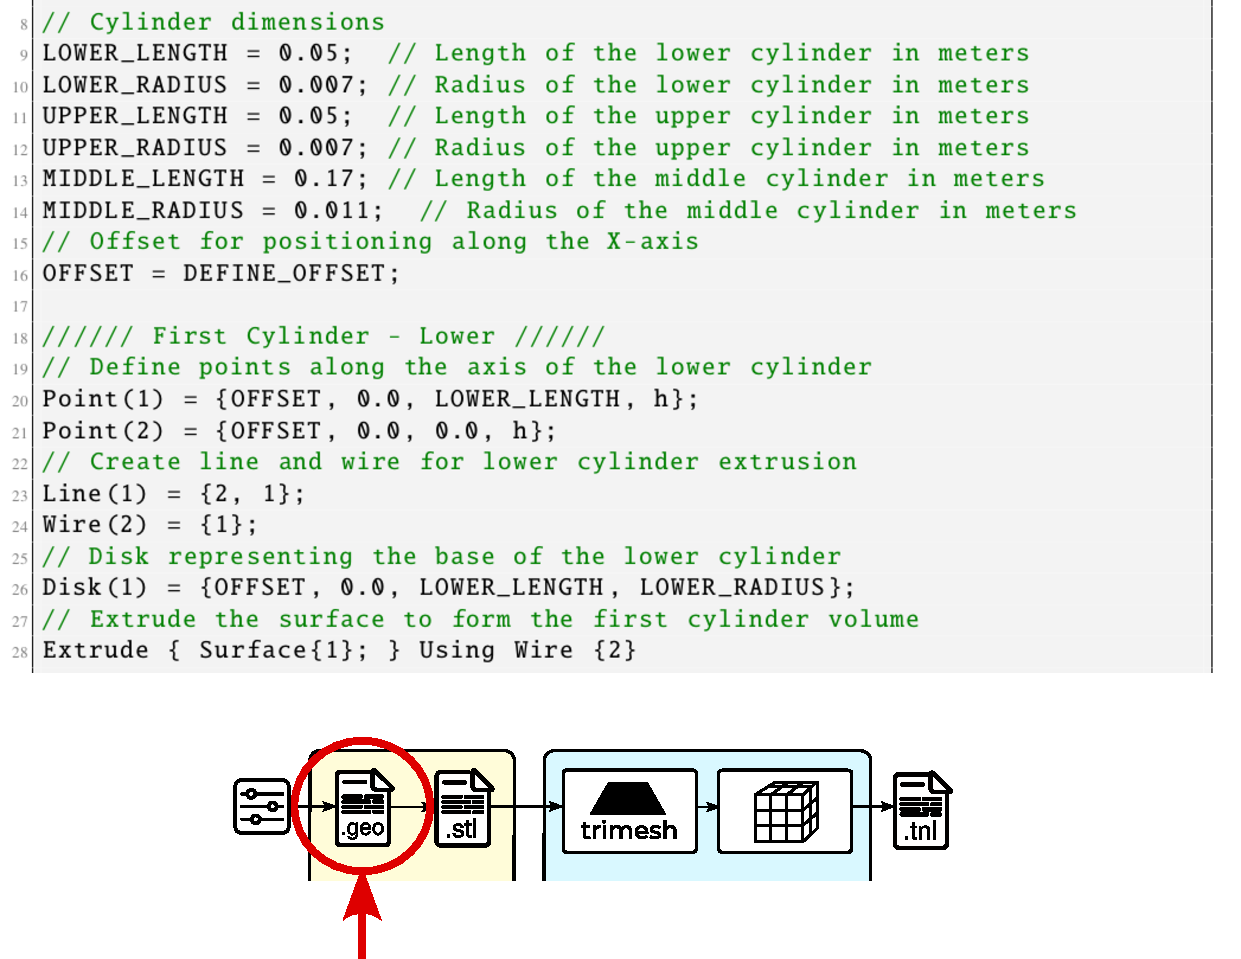
\includegraphics[width=0.6\linewidth, trim={0 -0.1cm 0 0}, clip]{Images/meshgen-1.pdf}
	\end{figure}
\end{frame}
%------------------------------------------------
\begin{frame}{Generování geometrie - STL}
	\begin{figure}
		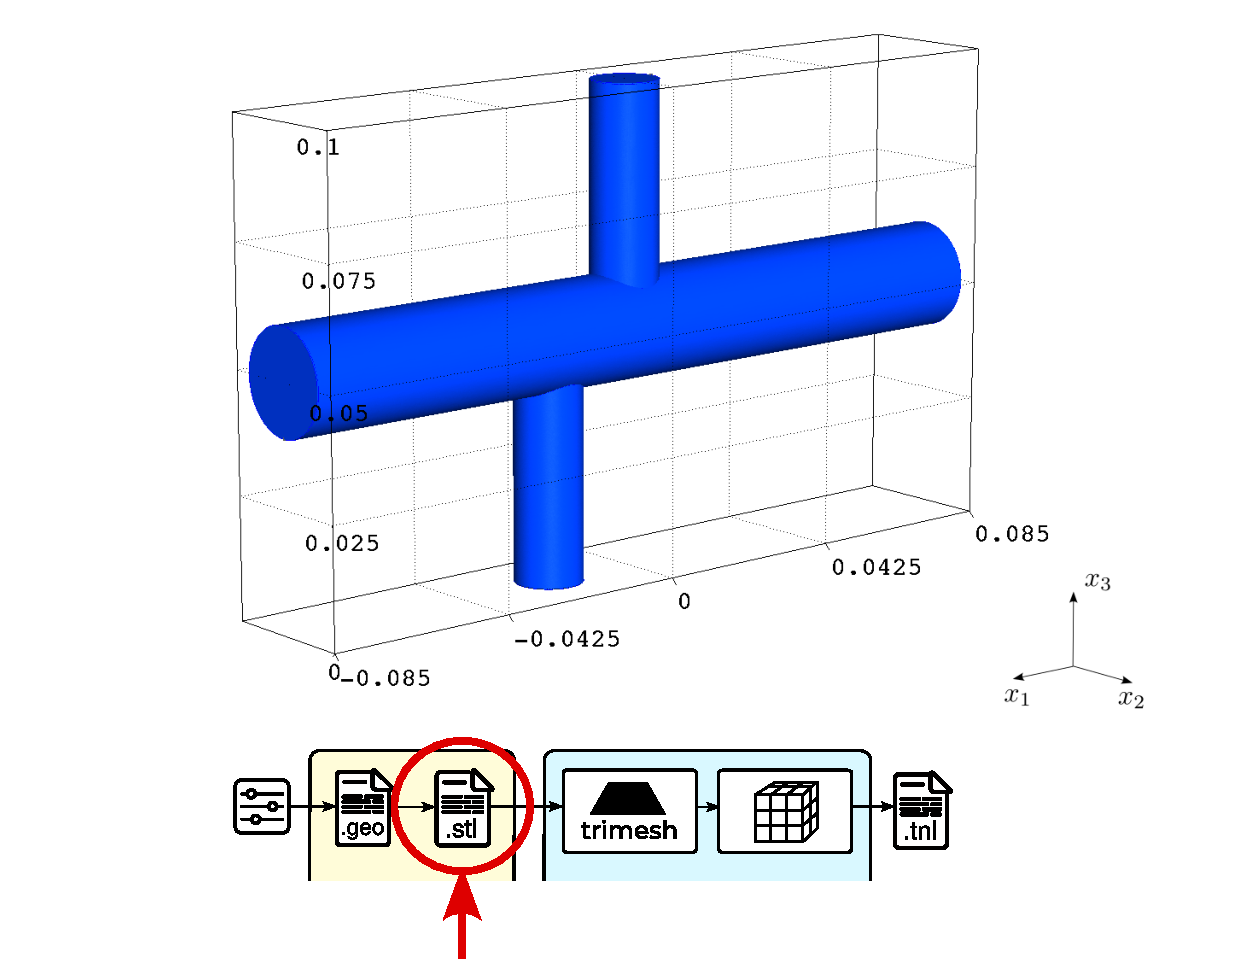
\includegraphics[width=0.6\linewidth, trim={0 -0.1cm 0 0}, clip]{Images/meshgen-2.pdf}
	\end{figure}
\end{frame}
%------------------------------------------------
\begin{frame}{Generování geometrie - voxelizace}
	\begin{figure}
		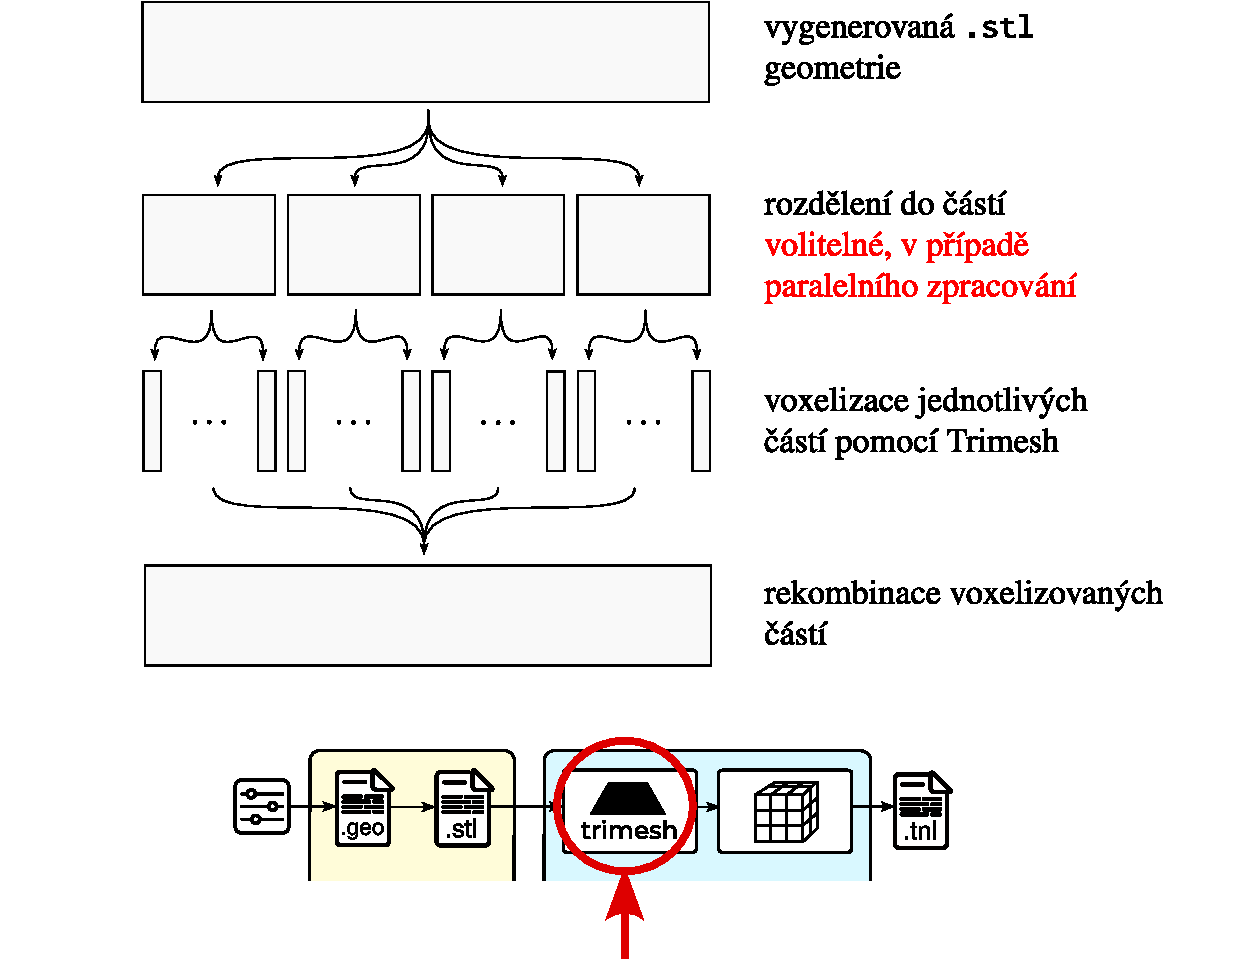
\includegraphics[width=0.6\linewidth, trim={0 -0.1cm 0 0}, clip]{Images/meshgen-3.pdf}
	\end{figure}
\end{frame}
%------------------------------------------------
\begin{frame}{Generování geometrie - výsledek}
	\begin{figure}
		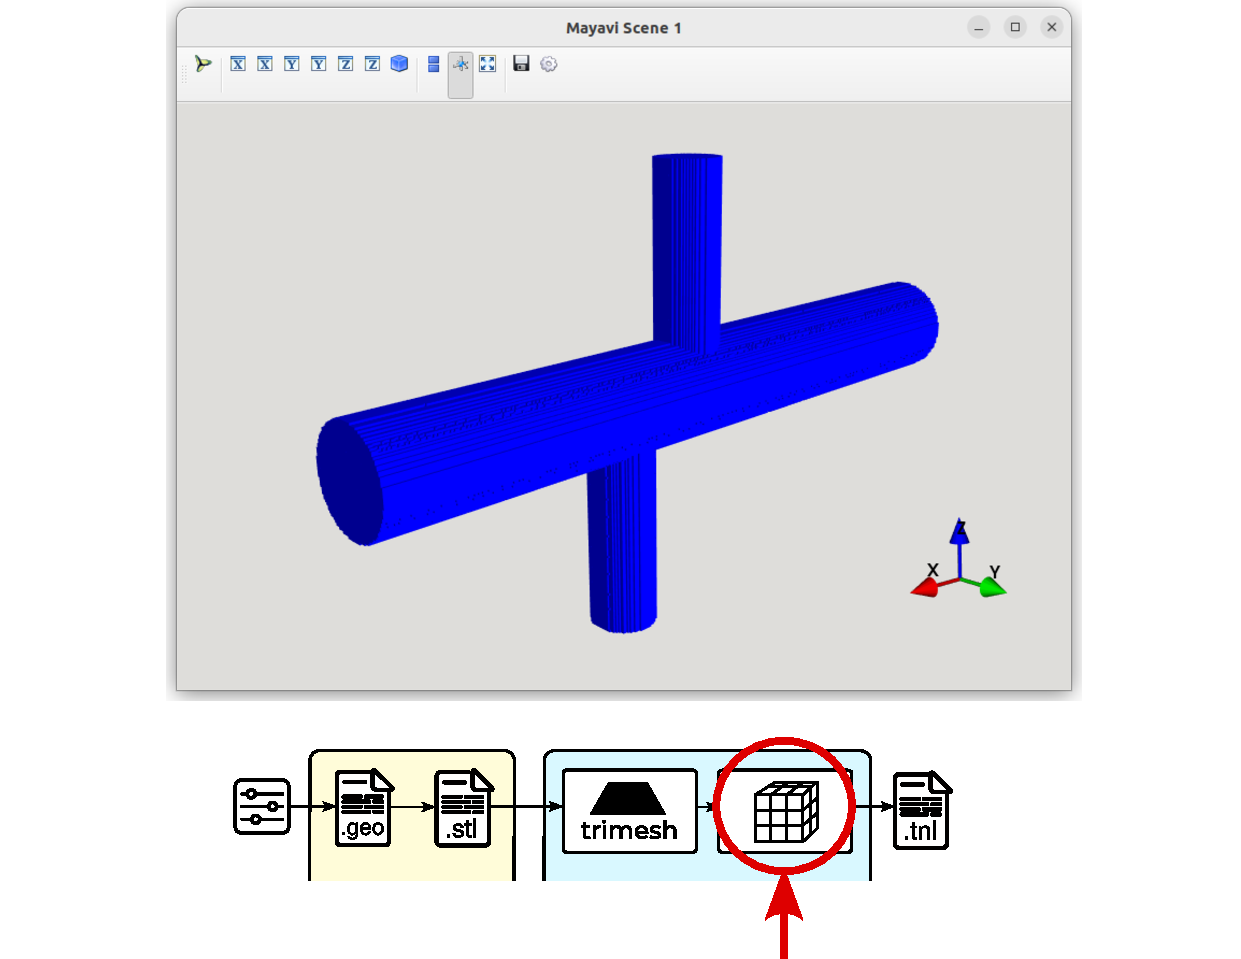
\includegraphics[width=0.6\linewidth, trim={0 -0.1cm 0 0}, clip]{Images/meshgen-4.pdf}
	\end{figure}
\end{frame}
%------------------------------------------------
\begin{frame}{Rámec}
	\addtocounter{framenumber}{-1}
	\begin{figure}
		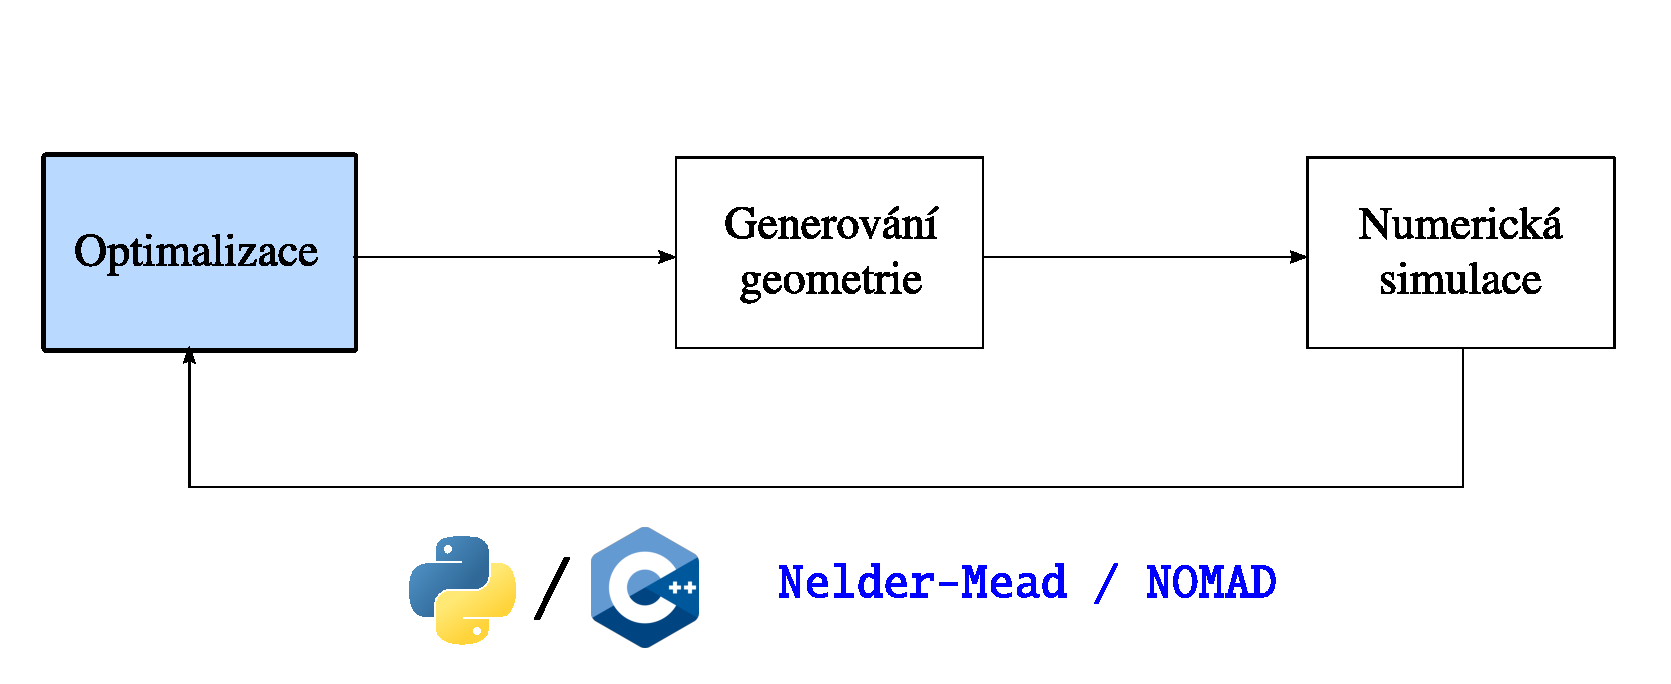
\includegraphics[width=0.95\linewidth, trim={0 -0.1cm 0 0}, clip]{Images/framework-cz-3.pdf}
	\end{figure}
\end{frame}

%------------------------------------------------
\begin{frame}{Optimalizace}
	\begin{itemize}
		\setlength\itemsep{1.8em}
		\item Předchozí práce (VÚ) $\Rightarrow$ bezgradientní metody
		\item Úloha s vazbami $\Rightarrow$ extrémní bariérová metoda
		\item Vyčíslení $ f \ (x \, ) $ pomocí LBM $\Rightarrow$ \alert{výpočetně i časově náročné}
		\item Algoritmy:
			 \begin{itemize}
				\item[-] Nelderova-Meadova metoda -- vlastní implementace \alert{podporující paralelizaci}
				\item[-] Mesh Adaptive Direct Search (NOMAD [1])
			 \end{itemize}
	\end{itemize}
\vspace{5.5mm}
\tiny{[1] C. Audet, et al. (2022)}, \textit{Algorithm~1027: NOMAD version~4: Nonlinear optimization with the MADS algorithm.}, DOI: 10.1145/3544489\\
\end{frame}



%------------------------------------------------
\section{Výsledky}
%------------------------------------------------
\begin{frame}{Výsledky}
	\begin{itemize}
		\setlength\itemsep{1.4em}
		\item Použití balíku \texttt{meshgen}, řešení netriviálních úloh
		\item Reynoldsův rozklad:
				$$ \vect{u} \,(x, y, z, t) = \overline{\vect{u} \,(x, y, z)} + \vect{u}^\prime(x, y, z, t) $$
		\item Účelové funkce: turbulentní kinetická energie a smyková rychlost
				$$ T_{\mathrm{turb}} = \frac{1}{2} (\vect{u}^\prime(x, y, z, t) )^2, \hspace{5mm} \dot{\gamma} = \sqrt{2} || \, \mathbf{D} \, ||^{}_{F}$$
		\item Nestlačitelná newtonovská tekutina, 3D
	\end{itemize}
\end{frame}

%------------------------------------------------
\begin{frame}{Idealizovaný model TCPC}
	\begin{center}	
		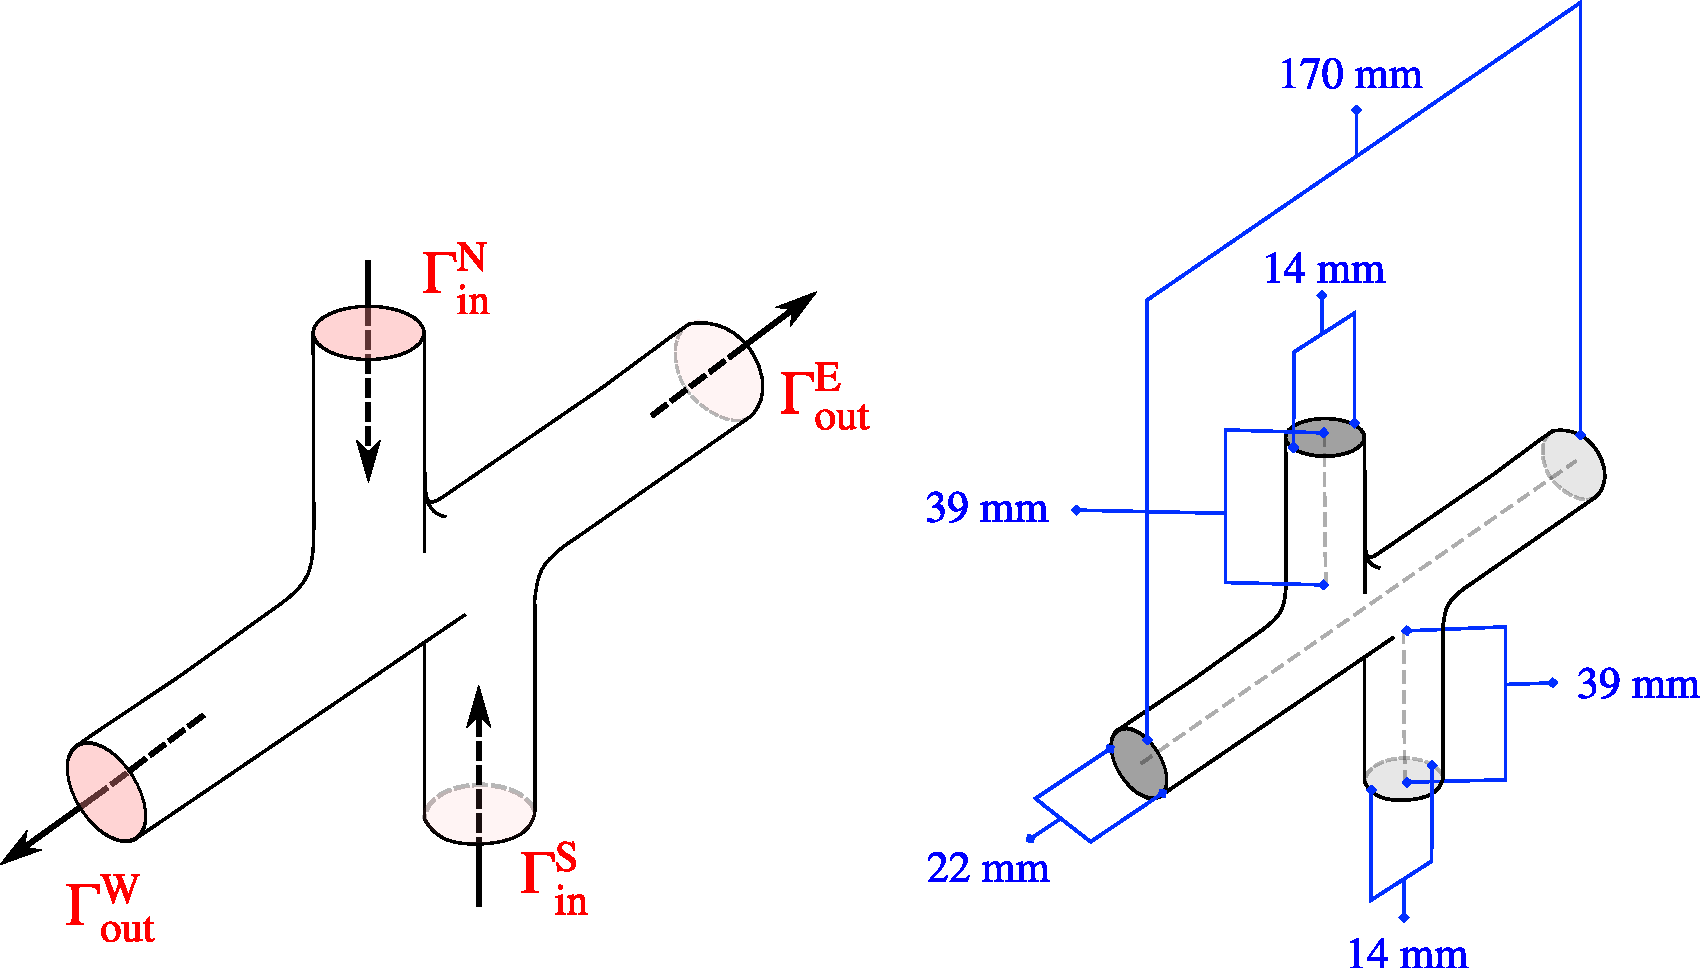
\includegraphics[width=0.7\linewidth, trim={0 0 0 0}, clip]{Images/3d-tcpc-schema-combined.pdf}	
	\end{center}		
\end{frame}
%------------------------------------------------
\begin{frame}{1 parametr - posun IVC}
	\begin{itemize}
		\item Posun osy IVC, ozn. $o_1$, je jediný optimalizační parametr
	\end{itemize}
	\begin{center}
		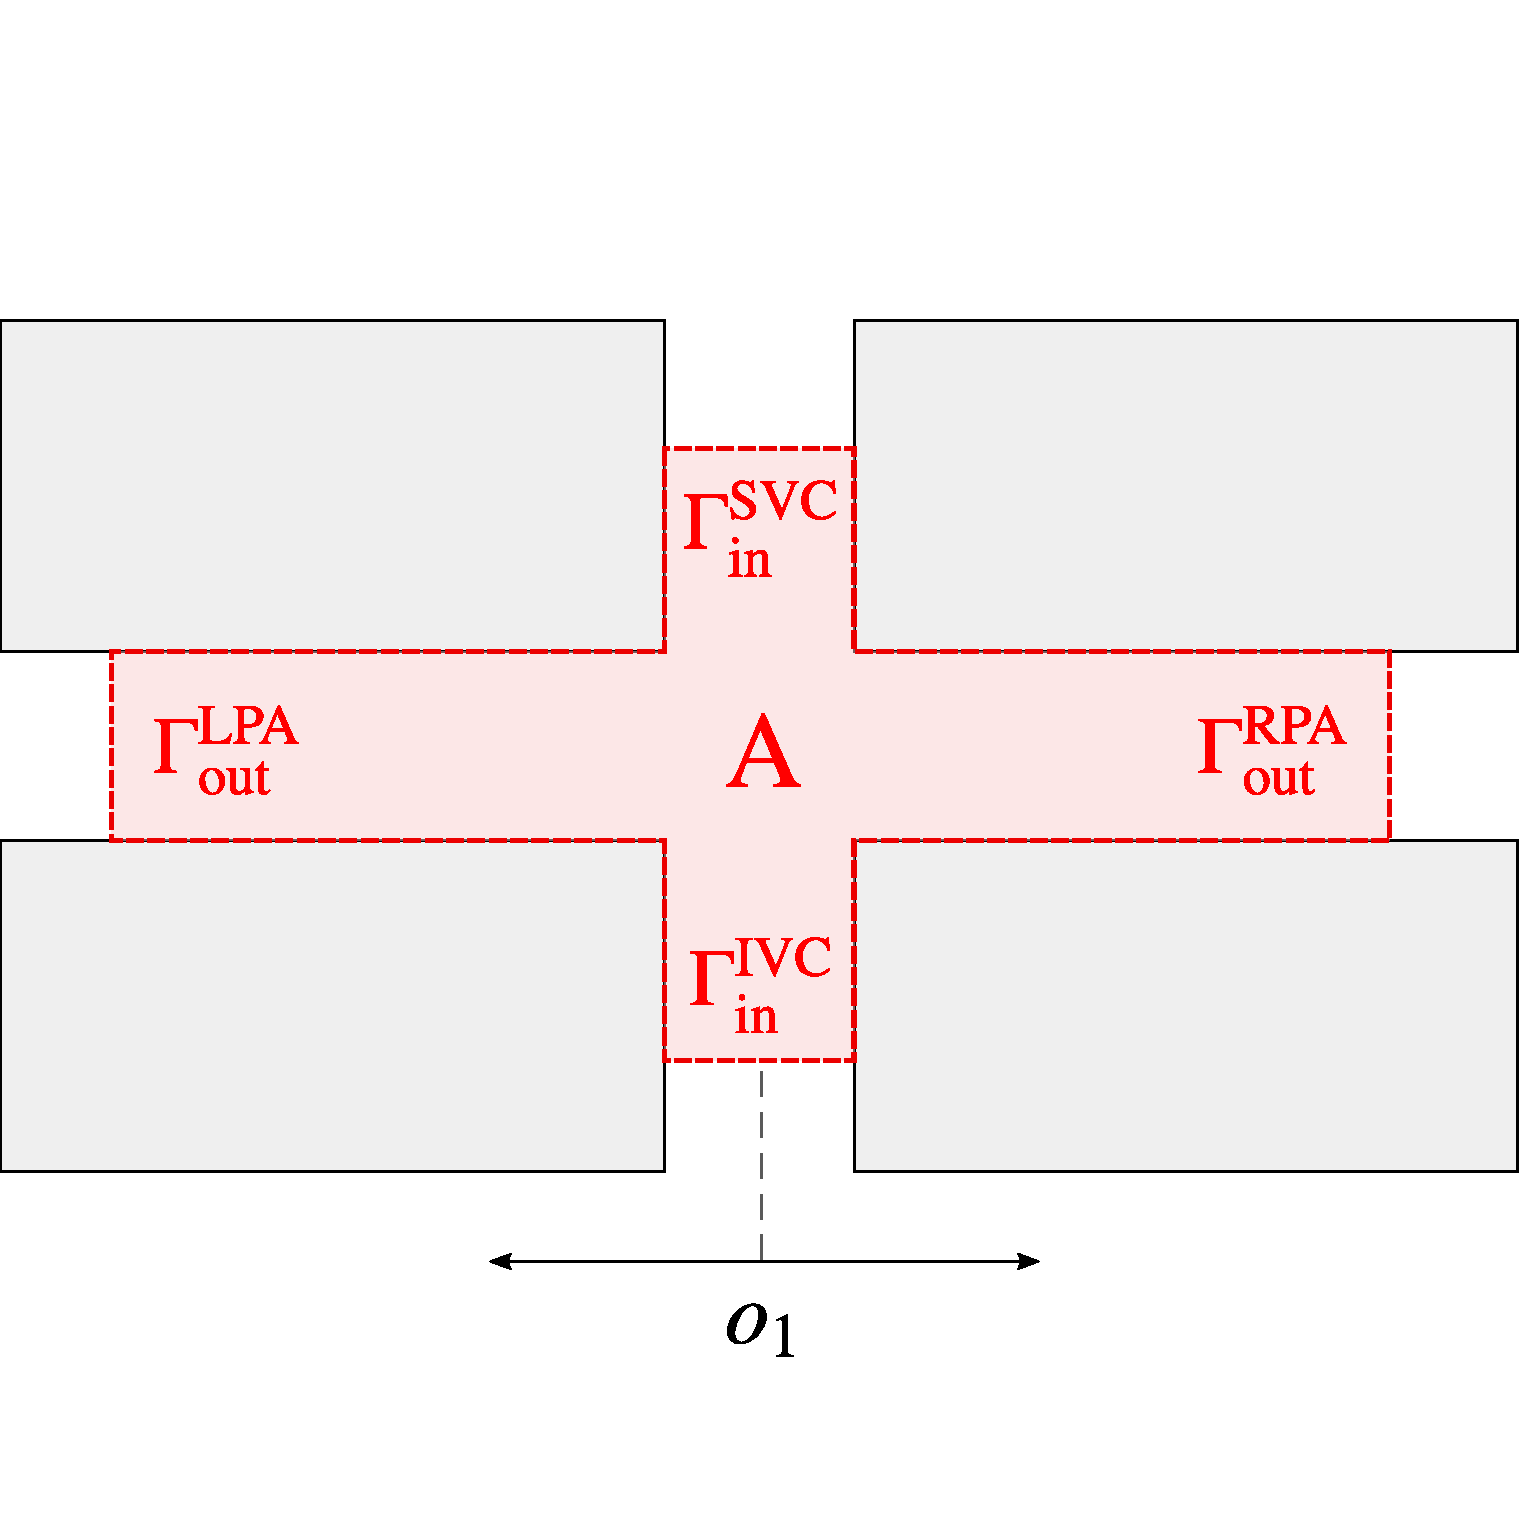
\includegraphics[width=0.55\linewidth, trim={0 0 0 36mm}, clip]{Images/model1.pdf}
	\end{center}			
\end{frame}
%%------------------------------------------------
\begin{frame}{1 parametr - účelové funkce}
	\begin{itemize}
		\item Účelových funkce v závislosti na posunu $o_1$ (vazba určená dělením IVC proudění)
	\end{itemize}
	\begin{columns}
		\begin{column}{.5\textwidth}
			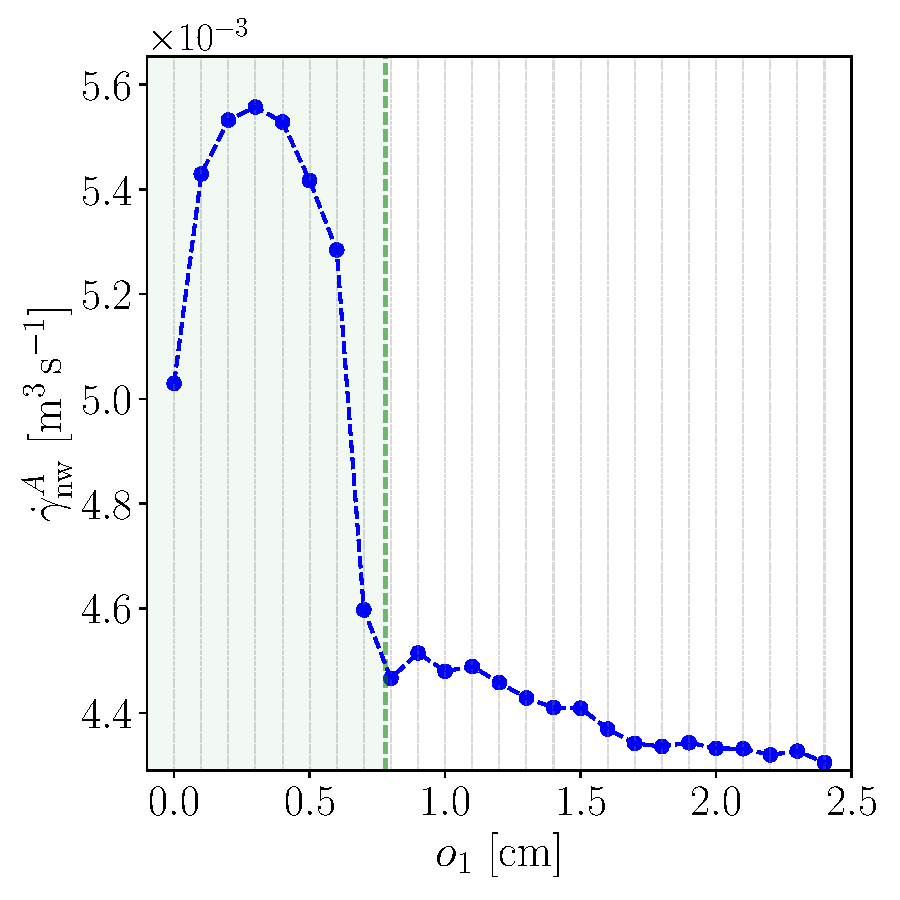
\includegraphics[width=0.9\linewidth, trim={0 0 0 0}, clip]{Images/mean_stress_3_interpolated.pdf}			
		\end{column}\hfill%
		\begin{column}{.5\textwidth}
			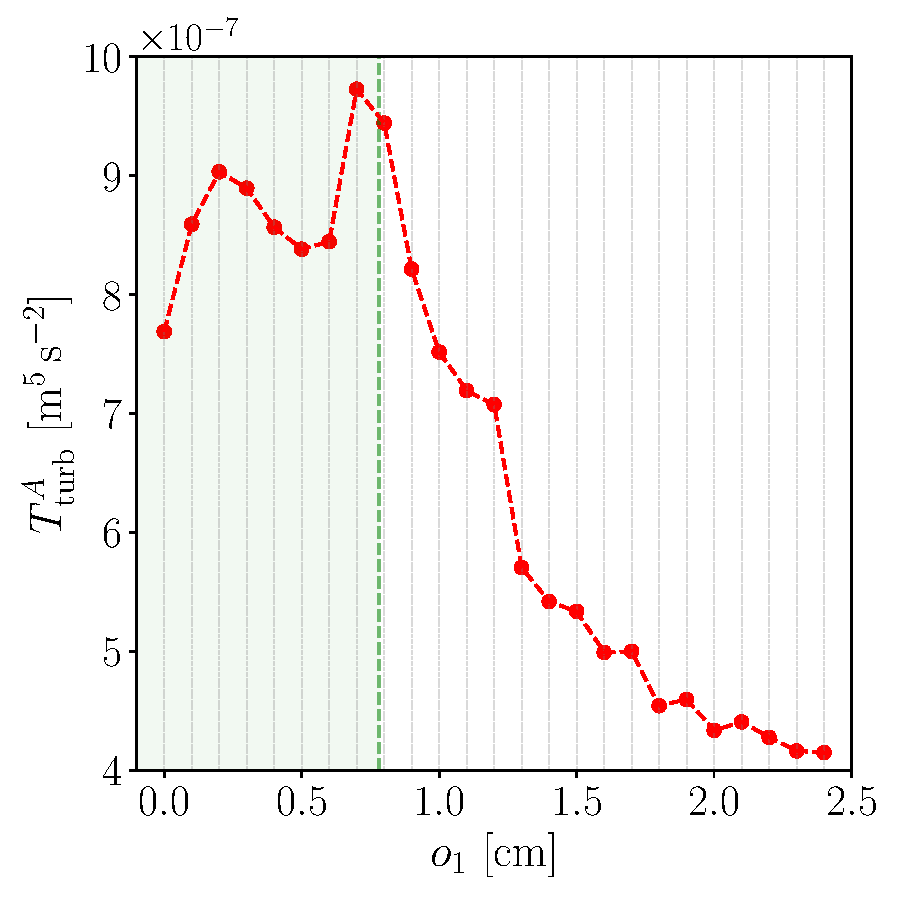
\includegraphics[width=0.9\linewidth, trim={0 0 0 0}, clip]{Images/mean_turbulence_kinetic_energy_interpolated.pdf}
		\end{column}
	\end{columns}
\end{frame}
%------------------------------------------------

\begin{frame}{1 parametr - výsledky}
	\begin{columns}
		\begin{column}{.5\textwidth}
			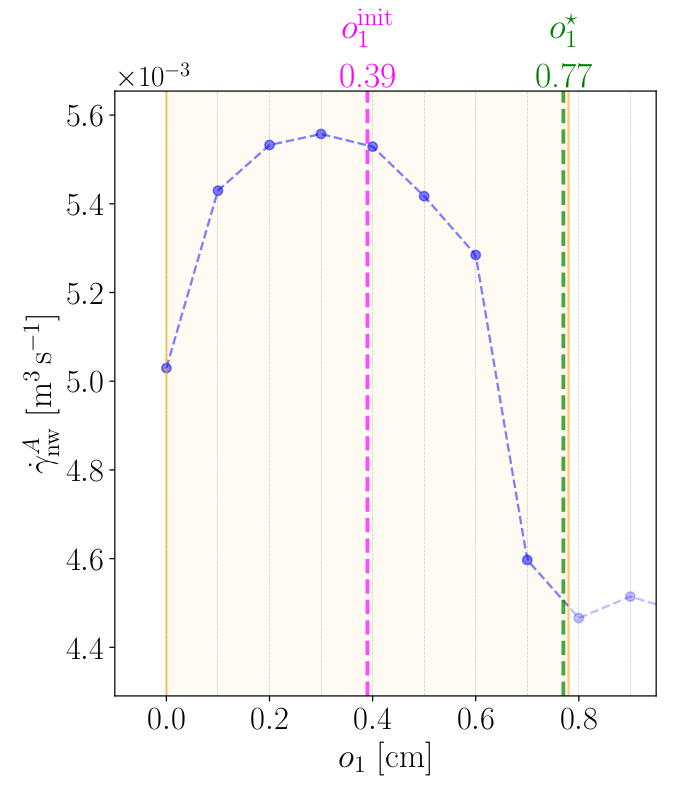
\includegraphics[width=0.7\linewidth, trim={0 0 0 3mm}, clip]{Images/problem1a.png}		
			\bgroup
			\tiny
			\centering
			\setlength\tabcolsep{5mm}
			\def\arraystretch{1.3}%
			\begin{tabular}{|c|c|c|}
				\hline
   				Metoda & Nelder-Mead & MADS \\ \hline
				Výpočetní čas [$h$] & 68.9 & 155.8 \\ \hline
			\end{tabular}
			\egroup	
		\end{column}
		\begin{column}{.5\textwidth}
			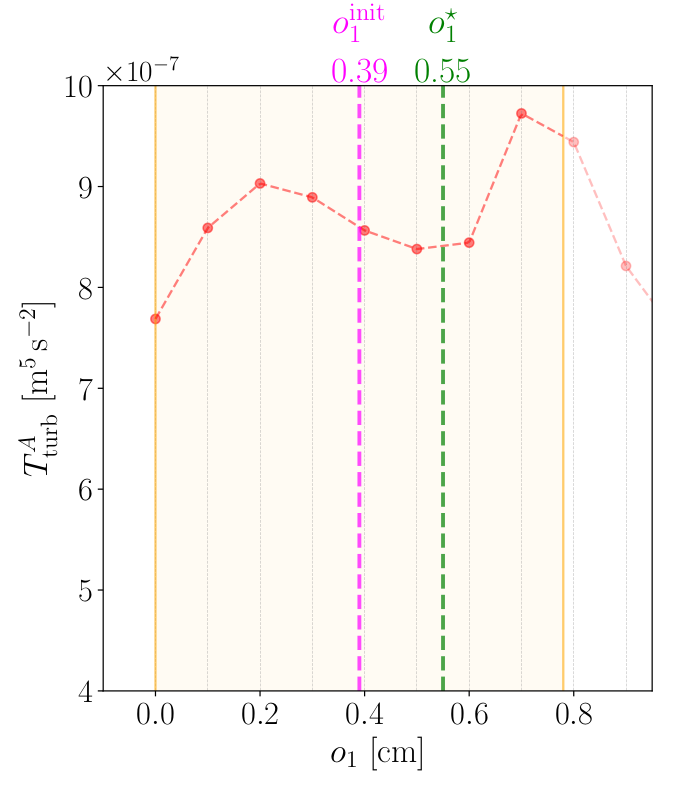
\includegraphics[width=0.7\linewidth, trim={0 0 0 1.5mm}, clip]{Images/problem1b.png}
			\bgroup
			\tiny
			\centering
			\setlength\tabcolsep{5mm}
			\def\arraystretch{1.3}%
			\begin{tabular}{|c|c|c|}
				\hline
				Metoda & Nelder-Mead & MADS \\ \hline
				Výpočetní čas [$h$] & 44.7 & 150.1 \\ \hline
			\end{tabular}
			\egroup	
		\end{column}
	\end{columns}
\end{frame}
%%------------------------------------------------
\begin{frame}{5 parametrů - model}
	
	\addtocounter{framenumber}{-1}
	\begin{itemize}
		\item Posun osy IVC, naklonění os dolního a horního kanálu, tvar napojení
	\end{itemize}
	\begin{center}
		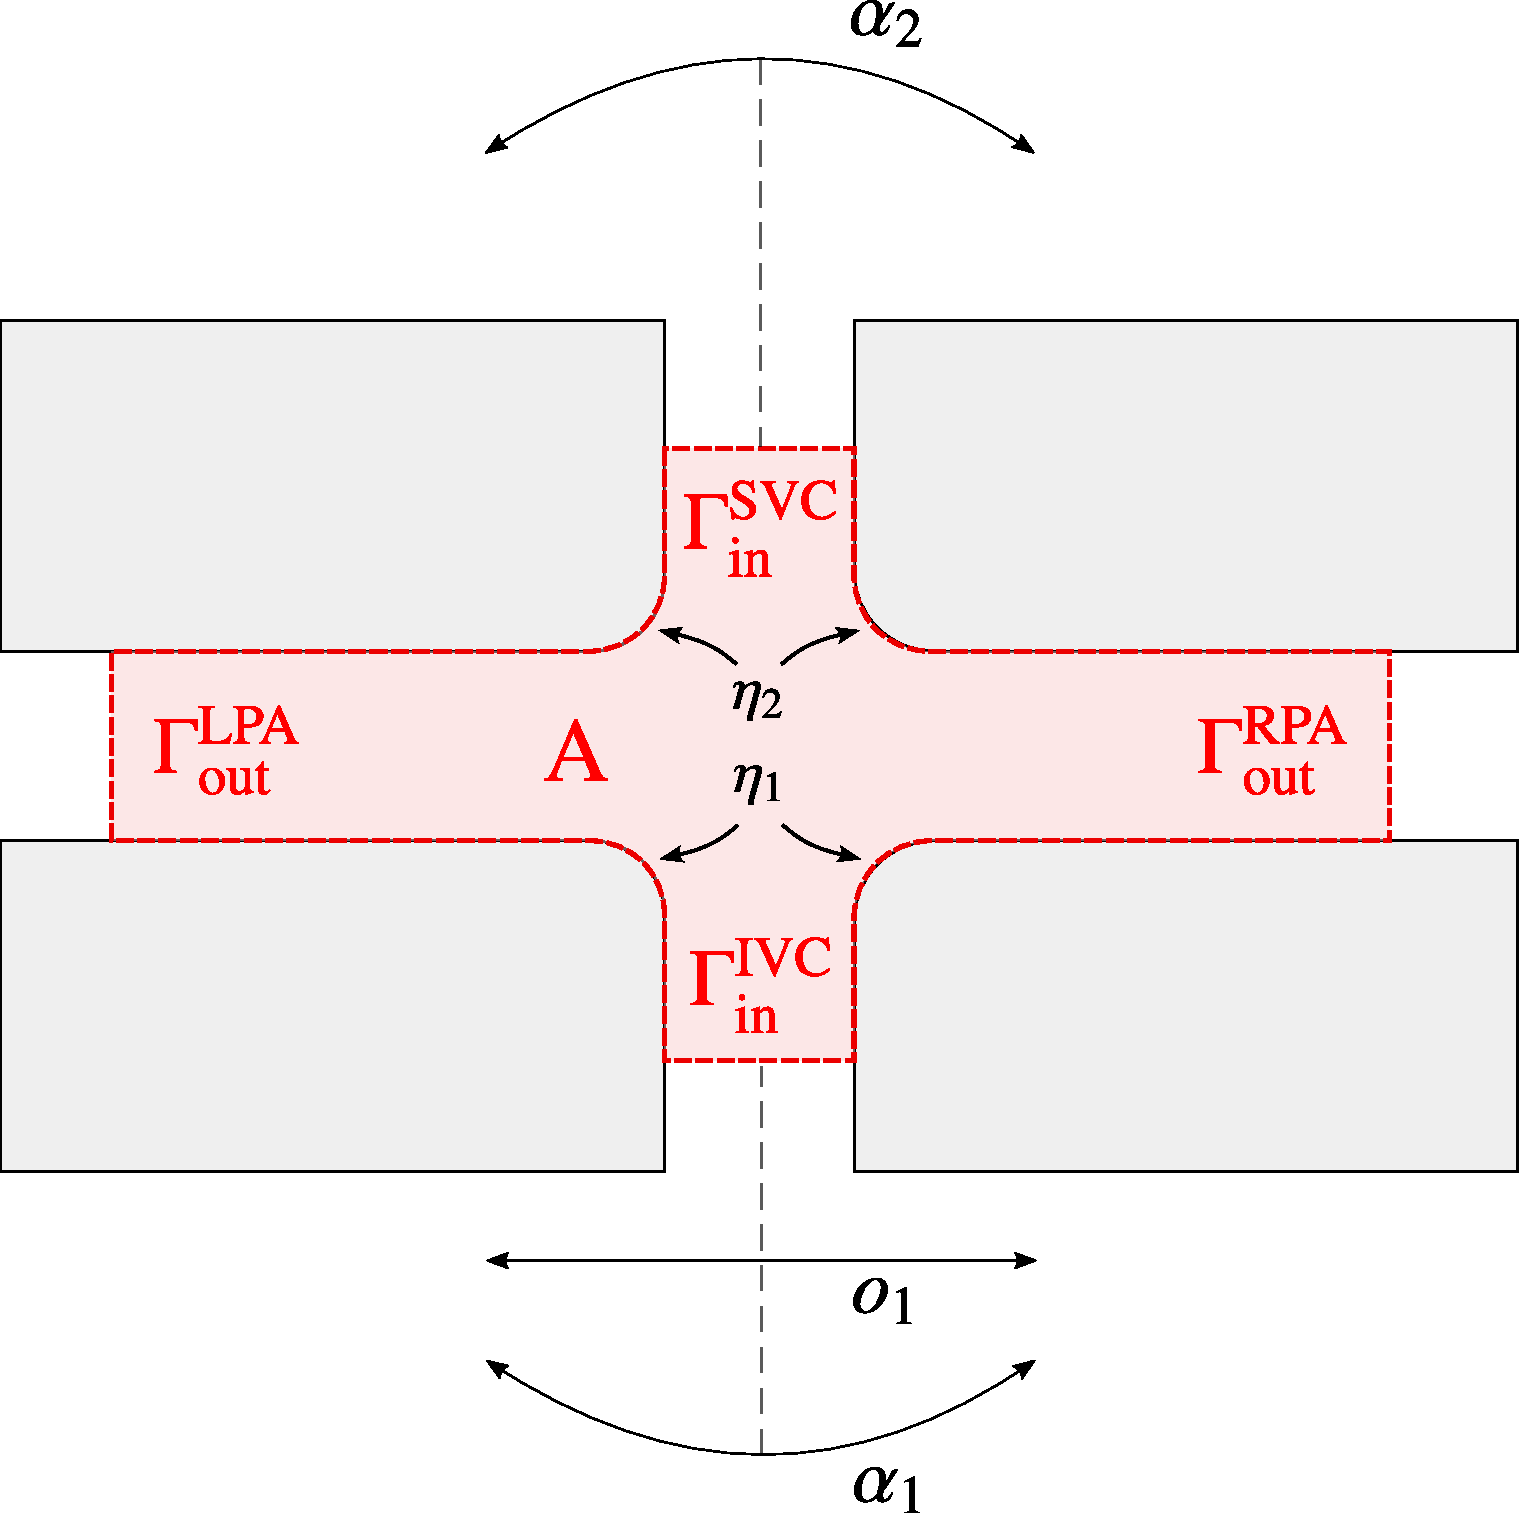
\includegraphics[width=0.45\linewidth, trim={0 0 0 0}, clip]{Images/model2.pdf}
	\end{center}
\end{frame}
%------------------------------------------------
\begin{frame}{5 parametrů - výsledky}
	
\begin{figure}
	\centering	
	\begin{subfigure}{0.5\textwidth}
		\centering
		{\textbf{NM}}\\[2pt]
		
		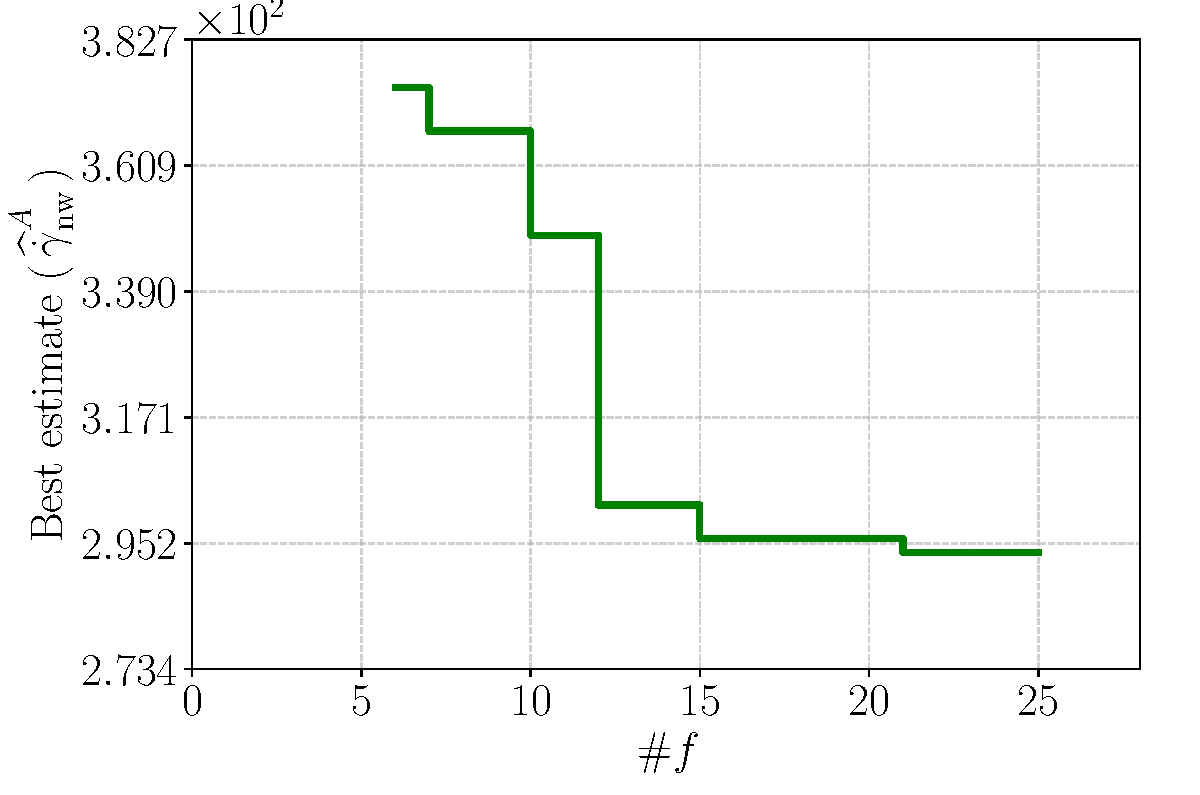
\includegraphics[
		width=\textwidth,
		trim={0mm 0mm 0mm 0mm}, clip
		]{Images/nm_sr_multi_crop.pdf}\\[5pt]
		\normalsize
	\end{subfigure}\hfill%
	\begin{subfigure}{0.5\textwidth}
		\centering
		{\textbf{MADS}}\\[2pt]
		
		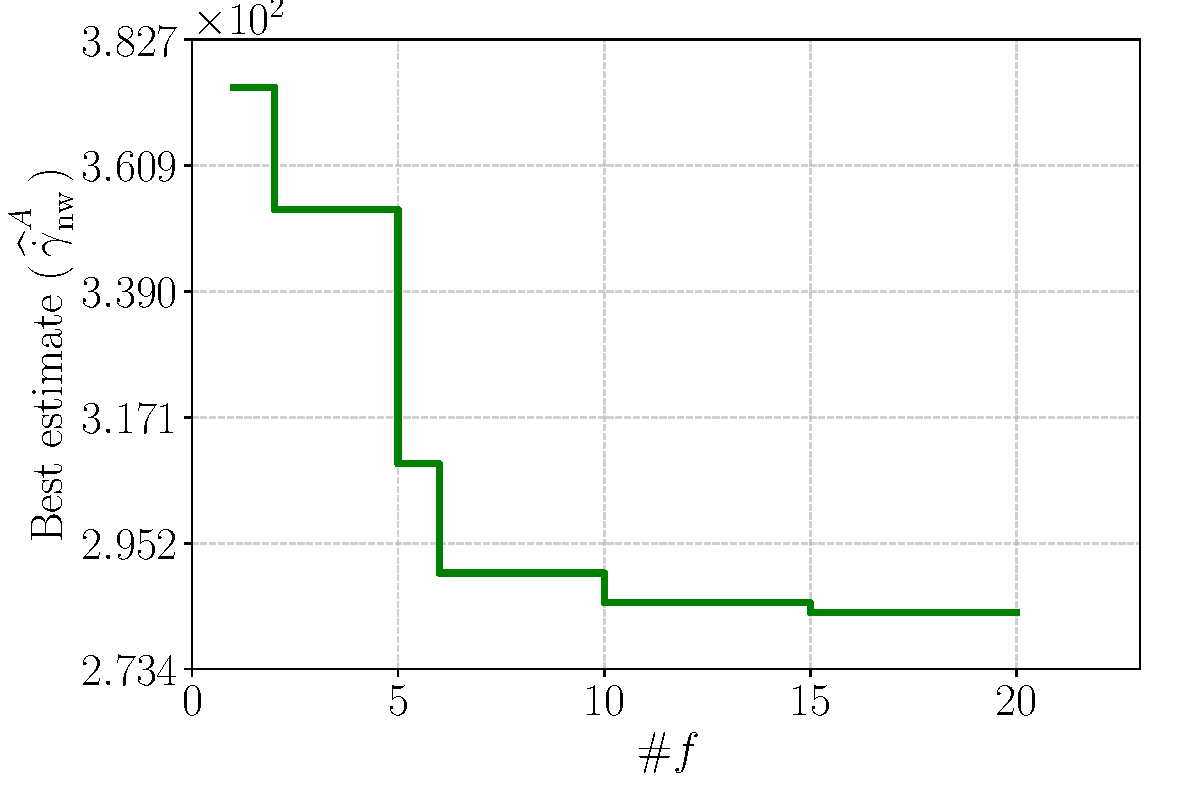
\includegraphics[
		width=1.0\textwidth,
		trim={0mm 0mm 0mm 0mm}, clip
		]{Images/mads_sr_multi_crop.pdf}\\[5pt]
		\normalsize
	\end{subfigure}
	\bgroup
	\scriptsize
	\centering
	\setlength\tabcolsep{3.5mm}
	\def\arraystretch{1.3}%
	\begin{tabular}{|c|c|c|c|c|c|c|c|}
		\multicolumn{6}{c}{} \\ \hline
		Řešení & Čas [$h$] & $o^{\mathrm{}}_1 \, [\mathrm{cm}]$ & $\alpha^{\mathrm{}}_1 \, [^\circ]$ & $\alpha^{\mathrm{}}_2 \, [^\circ]$ &  $\eta^{\mathrm{}}_1 \, [\mathrm{cm}]$ & $\eta^{\mathrm{}}_2 \, [\mathrm{cm}]$ \\ \hline
		$\mathbf{x^{\star}_\mathrm{NM}}$ & $\mathbf{49.2}$ & $-0.139$ & $ 6.8$ & $-0.2$ & $0.058$ & $ 0.128$ \\ \hline
		$\mathbf{x^{\star}_\mathrm{MADS}}$ & $\mathbf{144.2}$ & $0.1$ & $ 16$ & $13$ & $0$ & $ 0.25$ \\ \hline
	\end{tabular}
	\egroup
	\vspace{1mm}
	\caption{Convergence behavior,  a summary of the total elapsed time, and the optimal solutions $\vec{x^{\star}_\mathrm{NM}}$ and $\vec{x^{\star}_\mathrm{MADS}}$ obtained using the NM and MADS methods, respectively.
		%The plots illustrate the convergence behavior by showing the best estimate of the objective function value against $\# f$ (the number of evaluations of $f$). The table below the plots provides a summary of the total elapsed time and the comparison of the points identified as the optimal solution by the NM method ($\vec{x^{\star}_\mathrm{NM}}$) and the MADS method ($\vec{x^{\star}_\mathrm{MADS}}$).
	}
	\label{fig:optim results nd}
\end{figure}	
\end{frame}
%------------------------------------------------
\begin{frame}{5 parametrů - výsledky}
	
	\addtocounter{framenumber}{-1}
	\begin{center}
	
\includegraphics[width=0.95\linewidth, trim={0 0 0 0}, clip]{Images/popisky.png}
	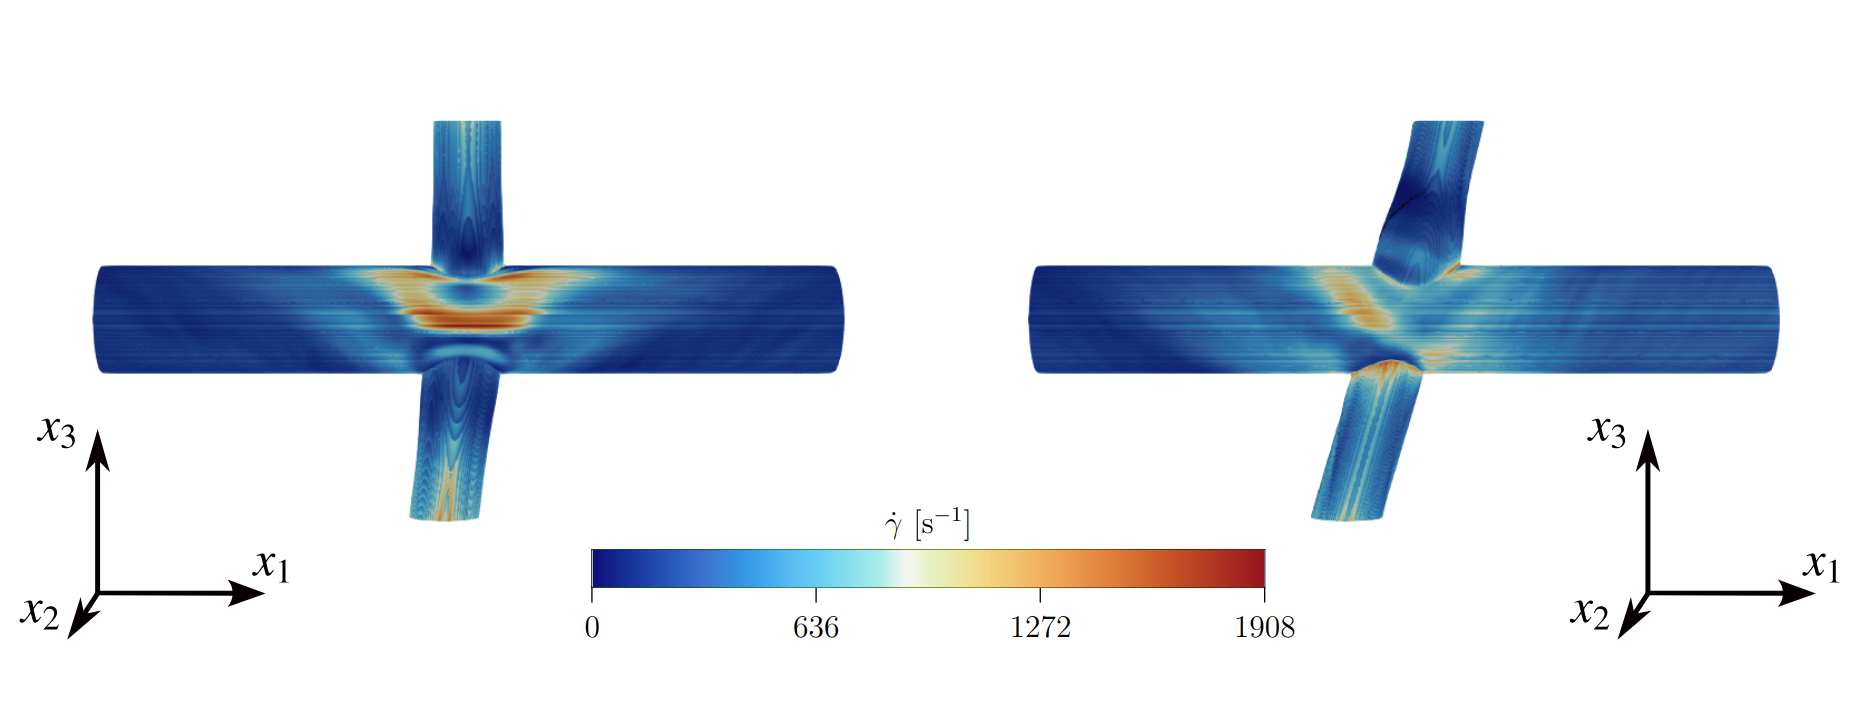
\includegraphics[width=0.95\linewidth, trim={0 0 0 0}, clip]{Images/smyk.png}
	\end{center}	
\end{frame}
%------------------------------------------------
\begin{frame}{5 parametrů - výsledky}
	
	\addtocounter{framenumber}{-1}
	\begin{center}
		
\includegraphics[width=0.95\linewidth, trim={0 0 0 0}, clip]{Images/popisky.png}
		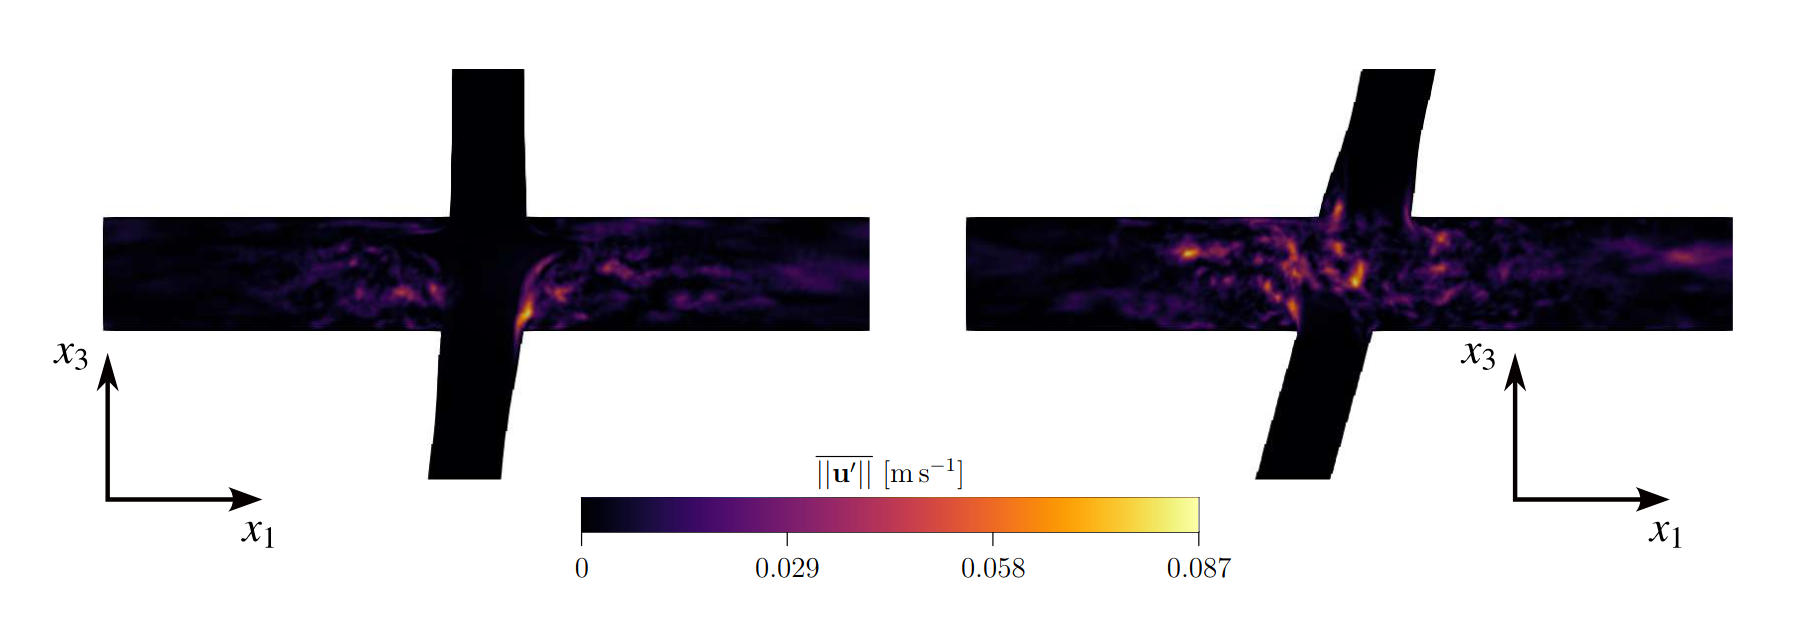
\includegraphics[width=0.99\linewidth, trim={0 0 0 0}, clip]{Images/fluc.png}
	\end{center}	
\end{frame}
%------------------------------------------------
\begin{frame}{5 parametrů - výsledky}
	
	\addtocounter{framenumber}{-1}
	\begin{center}
		
\includegraphics[width=0.95\linewidth, trim={0 0 0 0}, clip]{Images/popisky.png}
		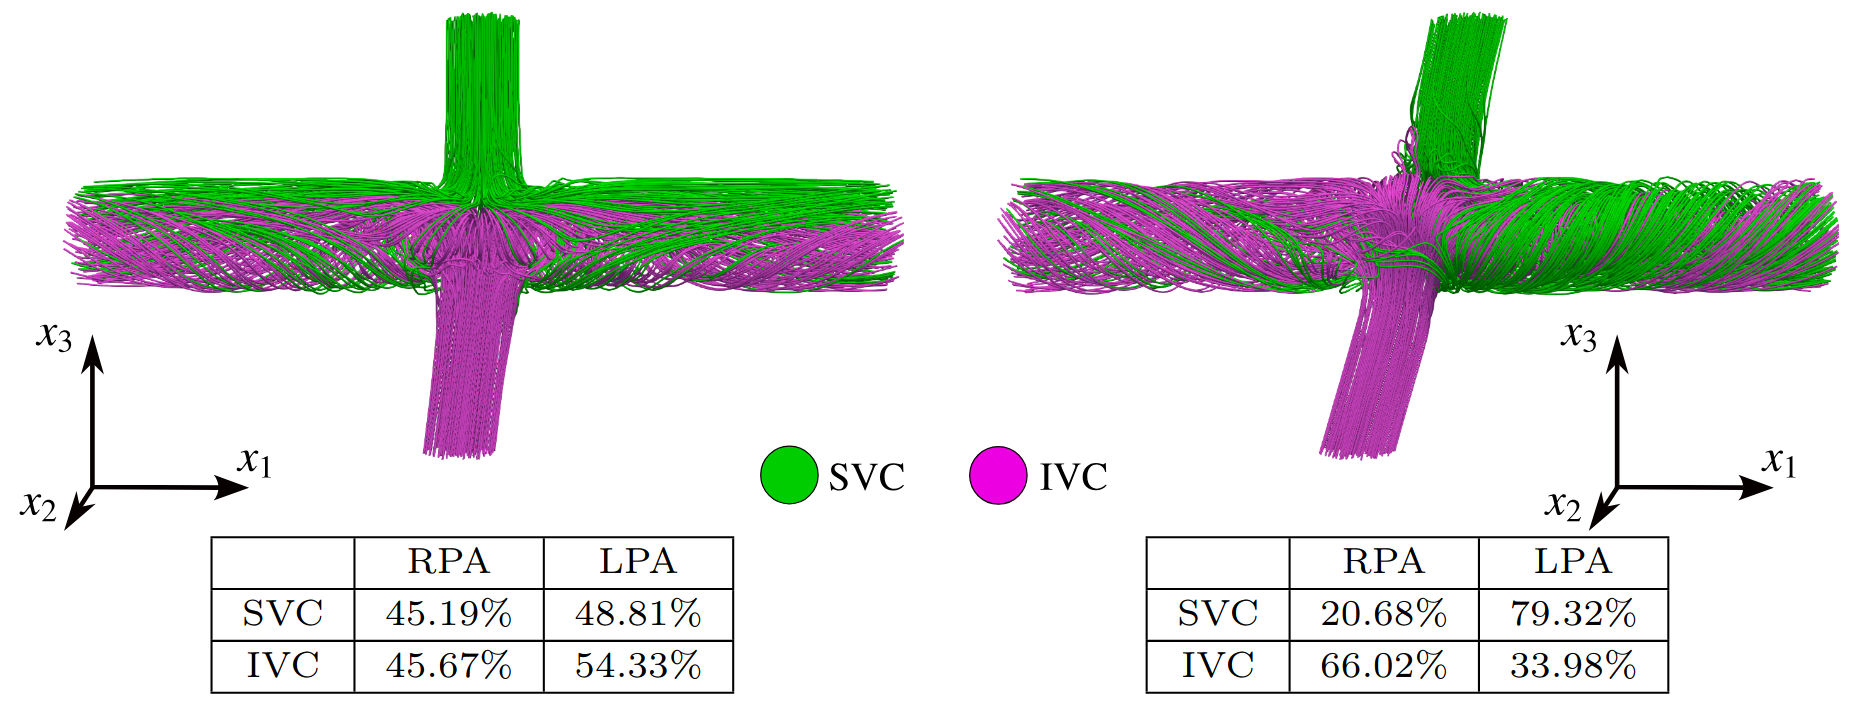
\includegraphics[width=0.99\linewidth, trim={0 0 0 0}, clip]{Images/split.png}
	\end{center}	
\end{frame}
%------------------------------------------------
\begin{frame}{5 parametrů - výsledky}
	
	\addtocounter{framenumber}{-1}
	\begin{center}
		
\includegraphics[width=0.95\linewidth, trim={0 0 0 0}, clip]{Images/popisky.png}
		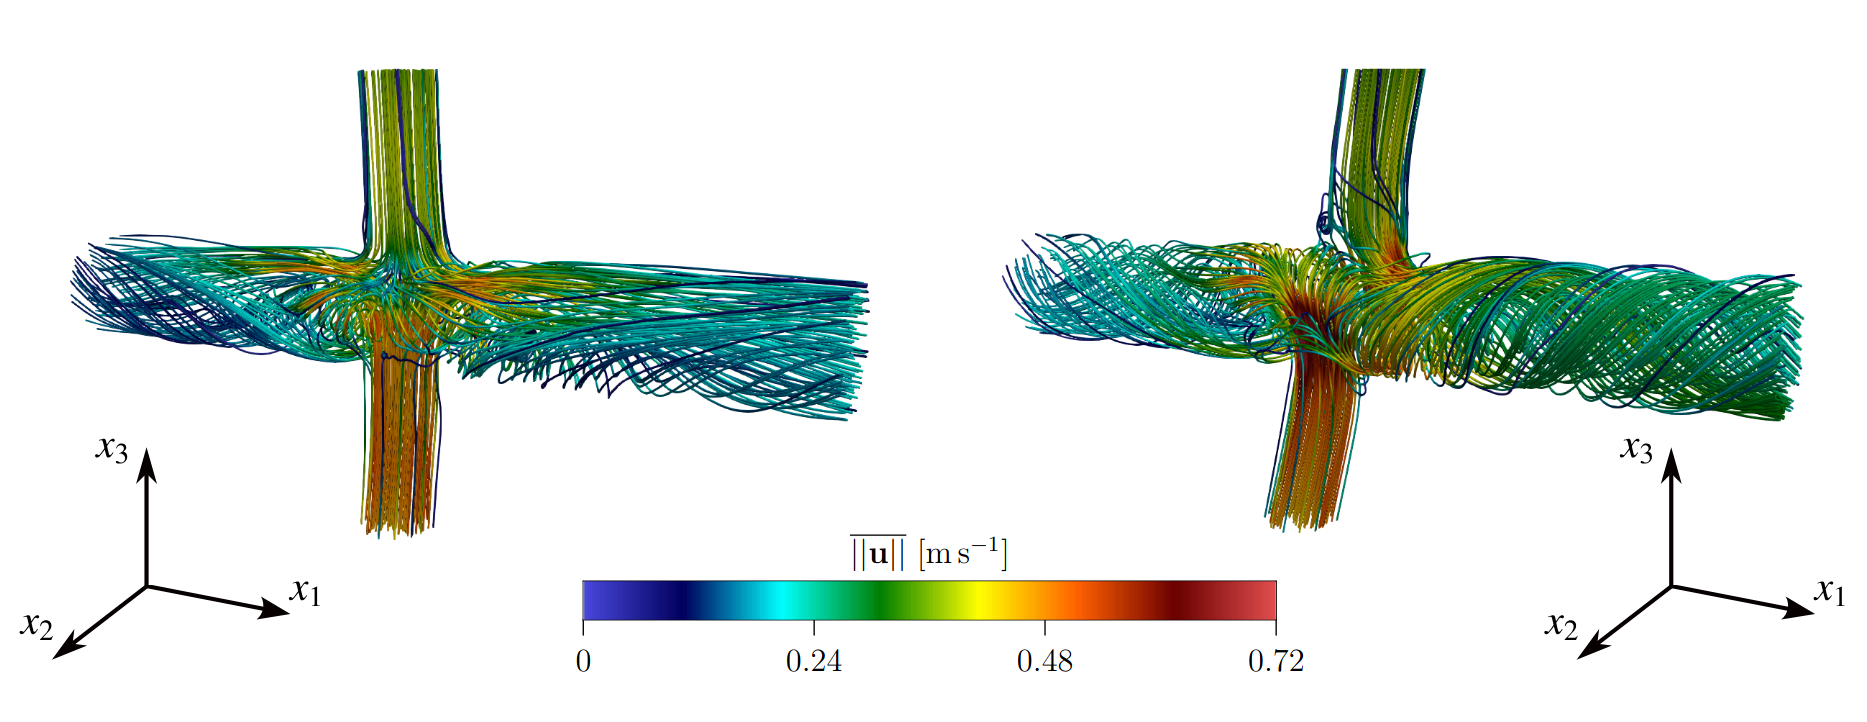
\includegraphics[width=0.99\linewidth, trim={0 0 0 0}, clip]{Images/streamlines.png}
	\end{center}	
\end{frame}

%%------------------------------------------------

\begin{frame}{Shrnutí}
%	\addtocounter{framenumber}{-1}
%	\setcounter{framenumber}{15}

	\begin{itemize}
		\setlength\itemsep{1.1em}
		\item Vytvořen rámec pro generování a řešení netriviálních optimalizačních úloh s pomocí LBM
		\item Navrženy parametrické modely idealizovaného TCPC
		\item Plány do budoucna (PGS):  zdokonalení rámce, reálná data, experimenty na MRI
		\item Publikace:\\[5pt]
		\begin{itemize}
			\item "Geometry optimization of idealized total	cavopulmonary connection using a CFD-based framework," \textit{FIMH 2025, Dallas} - podáno\\[5pt]
			\item Článek v přípravě
		\end{itemize}
	\end{itemize}
	\vfill%
	\huge{\centerline{\textbf{Děkuji za pozornost!}}}
\end{frame}
%------------------------------------------------
%%\begin{frame}{Zdroje}
%%    % Beamer does not support BibTeX so references must be inserted manually as below
%%    \footnotesize{
%%    	\begin{thebibliography}{99}
%%    		\bibitem[Smith, 2012]{p1} [1] Eichler P., Fučík R., Strachota P. (2022)
%%    		\newblock Investigation of mesoscopic boundary conditions for lattice Boltzmann method
%%    		in laminar flow problems.
%%    		\newblock preprint submitted to \emph{Comput. Math. with Appl.}.
%%    	\end{thebibliography}
%%    }
%%    \footnotesize{
%%        \begin{thebibliography}{99}
%%            \bibitem[Smith, 2012]{p1} [2] Bouzidi M., Firdaouss M., Lallemand P. (2001)
%%            \newblock Momentum transfer of a Boltzmann-lattice fluid with boundaries.
%%            \newblock \emph{Physics of Fluids} 13(11), 3452–3459.
%%        \end{thebibliography}
%%    }
%%	\vspace{1cm}
%%
%%	Všechny obrázky bez citace jsou originální nebo v public domain.
%%
%%\end{frame}
%
%
%%------------------------------------------------
\begin{frame}[plain,noframenumbering]{1. Hustota na přítoku OP}
%	\addtocounter{framenumber}{-1}
	\begin{itemize}
		\item Dotaz: \textit{Jak je nastavena/vypočítána hustota pro přítokovou okrajovou podmínku?}
		\item Na přítoku je použita rovnovážná (equilibrium) okrajová podmínka, kde se hustota fixuje na referenční hodnotu ($\rho=1 \, [-]$), rychlost se předepisuje konstatní.
		\item[]
		\item[]
		\item[]
		\item[]
		\item[]
		\item[]	
	\end{itemize}
\end{frame}
%------------------------------------------------
\begin{frame}[plain,noframenumbering]{2. Kritérium zastavení simulace}
	%	\addtocounter{framenumber}{-1}
	\begin{itemize}
		\item Dotaz: \textit{Jaké je přesné kritérium pro zastavení simulace proudění v LBM?}
		\item Je specifikovaný charakteristický čas $T$ stejný pro všechny simulace. Tento čas je volen tak, aby mohl být použit Reynoldsův rozklad.
		\item[]
		\item[]
		\item[]
		\item[]
		\item[]
		\item[]	
	\end{itemize}
\end{frame}
%%------------------------------------------------
\begin{frame}[plain,noframenumbering]{3. Nesymetrie symetrické úlohy}
	%	\addtocounter{framenumber}{-1}
	\begin{itemize}
		\item Dotaz: \textit{Co mohlo způsobit nesymetrii řešení jinak symetrické úlohy (je úloha opravdu symetrická i po diskretizaci?)}
		\item Výpočty prováděny s jednoduchou strojovou přesností, vliv by tedy mohla mít numerická chyba. Projektovaná geometrie je i po diskretizaci symetrická.\\[8pt]
		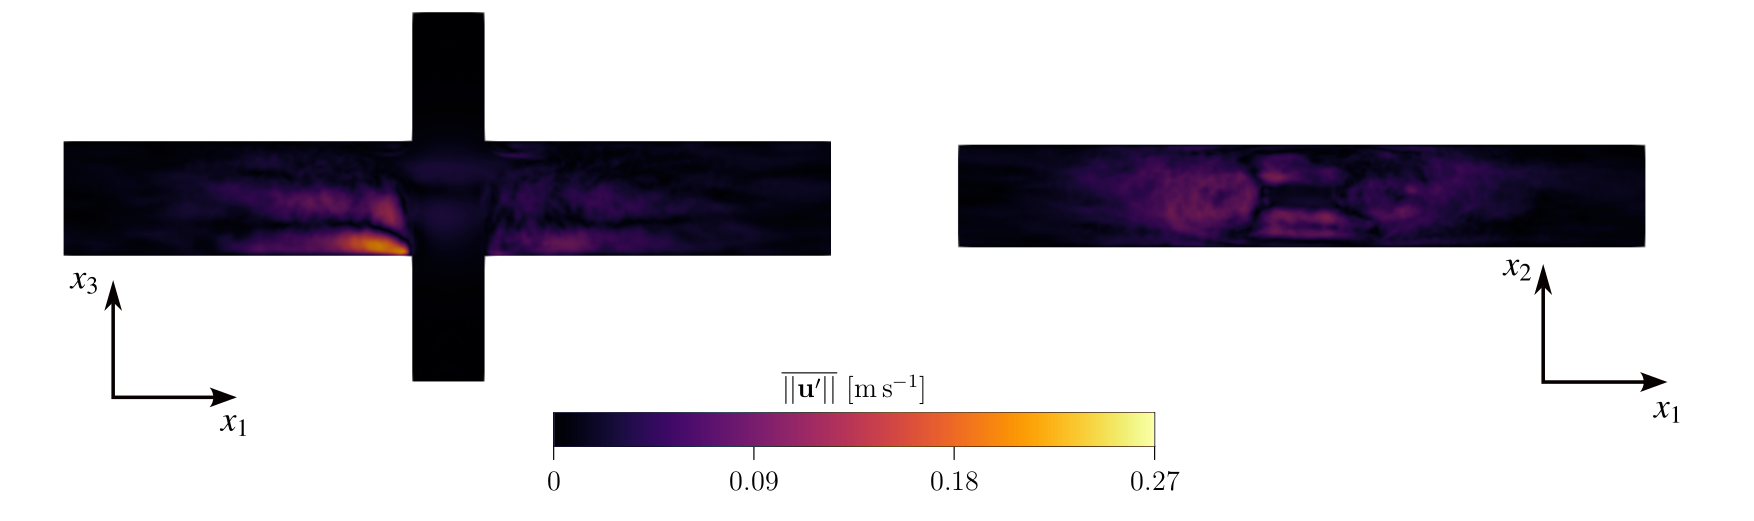
\includegraphics[width=0.99\linewidth, trim={0 0 0 0}, clip]{Images/dotaz.png}
	\end{itemize}
\end{frame}
%----------------------------------------------------------------------------------------
%------------------------------------------------
\begin{frame}[plain,noframenumbering]{4. Výpočet napětí na stěnách}
	%	\addtocounter{framenumber}{-1}
	\begin{itemize}
		\item Dotaz: \textit{Dal by se pro výpočet napětí na stěnách použít takový algoritmus, který používá M. Matyka?}\\[8pt]
		
\includegraphics[width=0.99\linewidth, trim={0 0 0 0}, clip]{Images/dotaz2.png}
	\end{itemize}
\end{frame}
%----------------------------------------------------------------------------------------
%------------------------------------------------
\begin{frame}[plain,noframenumbering]{5. Urychlení rámce}
	%	\addtocounter{framenumber}{-1}
	\begin{itemize}
		\item Dotaz: \textit{Dal by se optimalizační rámec více urychlit při zachování potřebného prostorového a časového rozlišení?}\\[8pt]
		\item Jistě je možné dále zefektivnit samotný  použitý optimalizační algoritmus. Dále je zde potenciál projektovat perturbovanou geometrii přímo za běhu jedné simulace, což by značně mohlo zkrátit čas potřebný k vyčíslení účelové funkce.
	\end{itemize}
\end{frame}
\end{document}